\documentclass[aps,prl,twocolumn,showpacs,amsmath,amssymb,superscriptaddress]{revtex4-1}

\usepackage{graphicx}
\usepackage[justification=centerlast]{caption} % FIXME: 'justified' should be default, but it does not work
\usepackage{subfig}
\usepackage{amsbsy}
\usepackage{amssymb}
\usepackage{esint}
\usepackage{bm}
\usepackage[usenames]{color}
\usepackage[shortcuts]{extdash}

\newcommand{\bogdansremark}[1]{\textcolor{red}{{[}BO: #1{]}}}
\newcommand{\petersremark}[1]{\textcolor{cyan}{{[}PD: #1{]}}}
\newcommand{\andreisremark}[1]{\textcolor{green}{{[}AS: #1{]}}}

% macros for different symbols
\newcommand{\Rb}{$^{87}$Rb}
\newcommand{\figref}[1]{Fig.~\ref{#1}}
\newcommand{\bra}[1]{\mbox{\ensuremath{\langle #1 |}}}
\newcommand{\ket}[1]{\mbox{\ensuremath{| #1 \rangle}}}
\newcommand{\xvec}{\boldsymbol{x}}
\newcommand{\ivec}{\boldsymbol{i}}
\newcommand{\jvec}{\boldsymbol{j}}
\newcommand{\kvec}{\boldsymbol{k}}
\newcommand{\Psivec}{\boldsymbol{\Psi}}

% Magic macro for creating tables in figure environment
\def\imagetop#1{\vtop{\null\hbox{#1}}}

\begin{document}

\title{ROUGH-DRAFT\_Quantitative simulations in three-dimensional atom interferometry}

\newcommand{\swinburneaffiliation}{ACQAO, Swinburne University of Technology, Hawthorn, VIC 3122, Australia}
\newcommand{\uqaffiliation}{ACQAO, Physics Department, University of Queensland, Queensland, Australia}

\author{B.~Opanchuk}
\affiliation{\swinburneaffiliation}
\author{M.~Egorov}
\affiliation{\swinburneaffiliation}
\author{S.~Hoffmann}
\affiliation{\uqaffiliation}
\author{A.~Sidorov}
\affiliation{\swinburneaffiliation}
\author{P.~D.~Drummond}
\affiliation{\swinburneaffiliation}

\begin{abstract}
We give a first-principles comparison of a calculation of quantum
phase-diffusion in a three-dimensional Bose gas,
as compared to recent experimental measurements.
Without using fitting parameters, we find excellent agreement
between the predicted fringe contrast and experimental data,
in an atom interferometer measurement.
\end{abstract}

\date{\today}

\maketitle

Atom interferometry is an important quantum technology,
at the heart of many suggested future applications of ultra-cold atomic physics.
Bose-Einstein condensates or atom lasers have potential advantages as detectors or sensors,
provided one can extract atomic phase information.
However, there is a challenge to be met.
Unlike photons, atoms can interact rather strongly, causing dephasing.
An intimate understanding of quantum many-body dynamics is essential in understanding
the precise nature of interaction-induced dephasing in the measurement process.
Progress in this technology therefore requires a quantitative theory of atom interferometry.

In this Letter we give a simple, yet quantitatively accurate
theoretical approach to calculations of atom interferometry at large atom number,
using a truncated Wigner representation.
This method extends the conventional Gross-Pitaevski equations
describing a Bose condensate to include quantum noise effects.
We show through comparison with experimental interferometric measurements on Bose condensates,
that the theory predicts observed dephasing results, within experimental errors.
No fitting parameters are required in these comparisons.
As a result, we suggest that the theoretical approach employed here
can be reliably used as a benchmark for predictions.
Importantly, we can clearly demonstrate where phase decay is driven by quantum fluctuations,
and where it is driven by trap inhomogeneity or other effects.

Quantum phase-diffusion is defined as the phase noise induced by number fluctuations,
which are intrinsically conjugate to phase.
As such, this is a fundamental limitation of any BEC interferometry,
and can only be removed when there are no interactions driving phase evolution.
However, there are other causes of density fluctuations as well as the overall number uncertainty,
which are also important in causing observed phase decays.
The important feature of the approach used here is that it is able to capture
all three significant features of atom interferometry that can result in decoherence.
These are:
\begin{itemize}
\item fluctuations caused by an atomic beam-splitter,
\item linear and nonlinear losses
\item trap inhomogeneity and propagation
\end{itemize}
We have not used variational or mean-field approximations.
Although these methods can certainly provide useful results,
they often require additional uncontrolled approximations.
Instead, the results given here simply require a controllable truncation
of an expansion in the inverse atom number.
They are applicable to simulations where the atom number per lattice point or mode is large.
Such quantitatively predictive theories have a great practical value
in assessing the utility of atom interferometry in new environments.
We expect that multi-configurational Hartree theories should give comparable or greater accuracy,
in principle, as they do not require truncation.
However, MCH methods are currently limited to lossless,
one-dimensional calculations with small atom numbers,
owing to computational complexity issues.

The theory we use is straightforward.
We start by assuming that the trapped BEC has S-wave interactions,
together with Markovian losses due to $n$-body collisions.
We employ the Wigner-Moyal quantum phase-space representation~\cite{Gardiner2004}
and the corresponding Lindblad-type master equation,
together with a truncation of third and higher-order derivatives in the equations of motion.
If we regard the commonly used Gross-Pitaevskii equation as a classical,
first approximation to mean-field condensate dynamics,
the truncated Wigner approach is best thought of as the second approximation
in an expansion in inverse particle number.
Such truncations have been shown to be valid in the limit of large particle number~\cite{Sinatra2002},
provided the effects of unoccupied vacuum modes can be neglected.
They are particularly useful in low-dimensional or trap environments,
where they have been succesful in predictions of quantum squeezing
and phase-diffusion effects to high accuracy in photonics~\cite{Corney2008}.
The truncation approximation has been further validated by comparison
with the exact positive-P method,
and with experiment in one-dimensional quantum soliton propagation dynamics.

In the present Letter, we treat an ultra-cold,
interacting multi-component spinor Bose gas in $D$ effective dimensions.
The basic Hamiltonian is easily expressed using quantum fields
$\widehat{\Psi}_{i}^{\dagger}(\xvec),\widehat{\Psi}_{j}(\xvec)$,
where $\widehat{\Psi}_{i}^{\dagger}(\xvec)$ creates a bosonic atom of spin $i$
at location $\xvec$, and $\widehat{\Psi}_{i}(\xvec)$ destroys one;
the commutators are
$[\widehat{\Psi}_{i}(\xvec),\widehat{\Psi}_{j}^{\dagger}(\xvec^\prime)] =
\delta^{(D)}(\xvec-\xvec^\prime)\delta_{ij}\,\,.$
The resulting physics of a dilute, low-temperature Bose gas
is well-described in the S-wave scattering limit by an effective Hamiltonian
with contact interactions and external potentials:
\begin{equation}
\begin{split}
	\widehat{H} / \hbar & = \int d^{D}\xvec \left\{
		-\frac{\hbar}{2m} \widehat{\Psi}_{i}^{\dagger} \nabla^2 \widehat{\Psi}_{i} +
		\omega_{ij}(t,\xvec) \widehat{\Psi}_{i}^{\dagger} \widehat{\Psi}_{j}
	\right\} \\
	& + \int d^{D}\xvec \left\{
		\frac{U_{ij}}{2} \widehat{\Psi}_{i}^{\dagger} \widehat{\Psi}_{j}^{\dagger}
		\widehat{\Psi}_{j} \widehat{\Psi}_{i}
	\right\} \,\,.
\end{split}
\end{equation}
Here we omit the field argument $(\xvec)$ for brevity,
and use the Einstein summation convention of summing over repeated indices.
Thus $\langle \widehat{\Psi}_{i}^{\dagger}(\xvec) \widehat{\Psi}_{i}(\xvec) \rangle$
is the spin $i$ atomic density, $m$ is the atomic mass,
and $U_{ij}$ is the atom-atom interaction term.
For a dilute gas at low enough temperatures,
$U_{ij}$ is related to the S-wave scattering length in three dimensions by:
\begin{equation}
	U_{ij}=\frac{4\pi\hbar a_{ij}}{m}.
\end{equation}
Here we implicitly assume a momentum cutoff $k_{c} \ll 1 / a_{ij}$,
otherwise the couplings must be renormalized~\cite{Sinatra2002}.
The linear coupling term is given by:
\begin{equation}
	\omega_{ij}(t,\xvec) = \left[
		\omega_{i} + V_{i}(\xvec) / \hbar
	\right] \delta_{ij} + \Omega_{ij}
\end{equation}
where $V_{i}$ is the external trapping potential for spin $i$,
$\omega_{i}$ is the internal Zeeman energy splitting associated with spin $i$,
and $\Omega_{ij}$ represents a time-dependent coupling
that is used to rotate one spin projection into another.

The truncated Wigner-Moyal quantum phase-space theory is well-suited
to these types of calculation of many-body dynamics.
Although the Wigner function is not a true probability,
its becomes one to a good approximation in the limit of large particle number,
so that a probabilistic (random) sampling of phase-space trajectories
can be used to treat quantum fluctuations.
This means that there are no complexity problems due to exponential growth
of the numbers of quantum states.
Furthermore, it is straightforward to treat a spatially inhomogeneous,
many-mode problem as found in an extended D-dimensional environment.
Initial conditions such as a coherent beam-splitter
as employed in typical atom interferometry experiments can be readily included.

This approach does require an approximation of truncating third-order derivatives
in an otherwise exact functional Fokker-Planck equation.
This approximation is valid when $N \gg M$, where $N$ is the atom number and
$M$ is the number of low-energy modes~\cite{Drummond1993,Sinatra2002,Norrie2006},
where it has been checked in one-dimensional cases.
We note that in free-space calculations in three dimensions,
the ultra-violet (UV) divergence in free-space mode density at large momentum cutoff
makes the truncated Wigner method unreliable,
unless a momentum truncation is used so that $N \gg M$.

In the relevant limits where the technique is applicable,
the equations simply reduce to Gross-Pitaevskii equations with Gaussian fluctuations
of the initial conditions and additional stochastic terms.
Damping and losses can be included via an additional Markovian master equation~\cite{Jack2002}
defined so that,
\begin{equation}
	\frac{d\hat{\rho}}{dt} = -\frac{i}{\hbar} \left[ \hat{H}, \hat{\rho} \right] +
	\sum_{n,\jvec} \kappa_{\jvec}^{(n)}
	\int d^D\xvec \mathcal{L}_{\jvec}^{(n)} \left[ \hat{\rho} \right],
\end{equation}
where $n$ is the number of interacting particles,
and $\jvec$ marks the subtype of the interaction (1--1, 1--2 and so on).

Here we introduce local Liouville loss terms,
\begin{equation}
	\mathcal{L}_{\jvec}^{(n)} \left[ \hat{\rho}\right] =
	2 \hat{O}_{\jvec}^{(n)} \hat{\rho}\hat{O}_{\jvec}^{(n)\dagger} -
	\hat{O}_{\jvec}^{(n)\dagger}\hat{O}_{\jvec}^{(n)}\hat{\rho} -
	\hat{\rho}\hat{O}_{\jvec}^{(n)\dagger}\hat{O}_{\jvec}^{(n)}
\end{equation}
where the reservoir coupling operators $\hat{O}_{\jvec}^{(n)}$
are all $n$-fold products of local field annihilation operators,
\begin{equation}
	\hat{O}_{\jvec}^{(n)} =
	\hat{O}_{\jvec}^{(n)} \left( \widehat{\Psivec} \right) =
	\widehat{\Psi}_{j_{1}} \left( \xvec \right)
	\widehat{\Psi}_{j_{2}} \left( \xvec \right) \ldots
	\widehat{\Psi}_{j_{n}} \left( \xvec \right)
\end{equation}
describing local $n$-body collision losses.
Ignoring unitary evolution, the corresponding mean amplitude equations
for an $n$-body loss of this form are:
\begin{equation}
	\frac{\partial}{\partial t} \left\langle
		\widehat{\Psi}_{i} \left( \xvec \right)
	\right\rangle =
	-\left\langle \hat{\Gamma}_{i} \left( \xvec \right) \right\rangle
\end{equation}
where we have introduced a nonlinear loss operator $\hat{\Gamma}_{i} \left( \xvec \right) =
\hat{\Gamma}_{i} \left( \widehat{\Psivec} \left( \xvec \right) \right)$ as:
\begin{equation}
	\hat{\Gamma}_{i} \left( \xvec \right) \equiv
	\sum_{n,\jvec} \kappa_{\jvec}^{(n)}
	\frac{\partial\hat{O}_{\jvec}^{(n)\dagger}	\left( \widehat{\Psivec} \right)}
		{\partial \hat{\Psi}_{i}^{\dagger} \left( \xvec \right)}
	\hat{O}_{\jvec}^{(n)} \left( \xvec \right) \,.
\end{equation}

As the full operator equations are highly nontrivial,
we proceed by using a stochastic phase-space method
that allows a numerical simulation of the condensate quantum dynamics~\cite{Drummond1993, Steel1998}.
Defining a Wigner function $W\left(\Psi_{1},\Psi_{2}\right)$,
where $\Psi$ is a c-number field corresponing to the quantum field $\hat{\Psi}$,
this corresponds to a time-evolution equation of form:
\begin{equation}
\begin{split}
	\frac{\partial W}{\partial t} & = \int d^D \xvec \,\left\{
		-\frac{\delta}{\delta\Psi_{i}} A_{i} -
		\frac{\delta}{\delta\Psi_{i}^*} A_{i}^* \right. \\
& + \left. \frac{\delta^{2}}{\delta\Psi_{i} \delta\Psi_{j}^{*}}D_{ij} +
		\mbox{O} \left[ \frac{\delta^{3}}{\delta\Psi_{i}^{3}} \right]
	\right\} W,
\end{split}
\end{equation}
% TODO:
%	\petersremark{The other way to proceed is to use a normalized field approach
%	with a normalization so that $\Psi \sim \epsilon\Psi$.
%	Then we can simply use a notation that the terms dropped are $O(\epsilon^3)$.
%	Here $\epsilon = \sqrt(M/N)$, say.
%	Then we must change the later notation as well, for consistency.}
where higher derivative terms of type $\mbox{O}\left[\delta^3/\delta\Psi_{i}^{3}\right]$
will be truncated.
This is equivalent to neglect of higher-order terms in an expansion in $1/\sqrt{N}$,
and is therefore valid in the limit of $N \gg M$.
The drift term $A_{i}$ corresponds to Gross-Pitaevskii type evolution,
with additional nonlinear damping:
\begin{equation}
	A_{i} = -i \left(
	 	-\frac{\hbar}{2m} \nabla^{2} + U_{ij} \left| \Psi_{j} \right|^{2}
	\right) \Psi_{i} -
	\hbar \omega_{ij} \Psi_{j} -
	\Gamma_{i} \left( \Psivec \right),
\end{equation}
where $\Gamma_{i}$ is a classical loss term:
\begin{equation}
	\Gamma_{i} = \sum_{n,\jvec} \kappa_{\jvec}^{(n)}
	\frac{
		\partial O_{\jvec}^{(n)*} \left( \Psivec \right)
	}{
		\partial \Psi_{i}^* \left( \xvec \right)
	}
	O_{\jvec}^{(n)} \left( \xvec \right)
\end{equation}

The next highest order term in the evolution equation gives rise to
quantum noise associated with the loss reservoirs,
with:
\begin{equation}
	D_{ij} = \sum_{n,\kvec} \kappa_{\kvec}^{(n)}
	\frac{\partial O_{\kvec}^{(n)*}}{\partial\Psi_{i}^{*}}
	\frac{\partial O_{\kvec}^{(n)}}{\partial\Psi_{j}}
\end{equation}

With the inclusion of reservoir couplings to describe losses
the truncated Fokker-Planck equation can be transformed
to a coupled stochastic Gross-Pitaevskii equation:
\begin{equation}
	\frac{d\Psi_{j}}{dt} = iK_{j} \Psi_{j} - iU_{ij} \lvert \Psi_{i} \rvert ^{2} \Psi_{j} -
	\Gamma_{j} + \sum_{n,\ivec} \gamma_{\ivec,j}^{(n)} \zeta_{\ivec}^{(n)} (\xvec,t)
\end{equation}

Here the linear unitary evolution of the wave-function, is described by:
\begin{equation}
	K_{j} = \hbar \nabla^{2}/2m - \omega_{j} - V_{j} \left( \xvec \right) / \hbar
\end{equation}
while $\zeta_{\ivec}^{(n)}(\xvec, t)$ is a complex,
stochastic delta-correlated Gaussian noise with
\begin{equation}
	\left\langle
		\zeta_{\ivec}^{(n)} (\xvec,t) \zeta_{\jvec}^{(m)}(\xvec^\prime, t^\prime)
	\right\rangle =
	\delta_{\ivec \jvec} \delta^{nm} \delta^{D} \left(
		\xvec - \xvec^\prime
	\right)
	\delta \left( t - t^\prime \right)\,.
\end{equation}
The multiplicative noise coefficient\---
\begin{equation}
	\gamma_{\ivec,j}^{(n)} \left( \Psivec \right) =
	\sqrt{\kappa_{\ivec}^{(n)}}
	\frac{\partial O_{\ivec}^{(n)}}{\partial\Psi_{j}}
\end{equation}
is needed as a fluctuation-dissipation term,
to ensure that the losses do not remove the vacuum fluctuations,
so that the Wigner variables remain equivalent to the corresponding operators.

For initial conditions in interferometry it is usually sufficient
to consider a coherent state amplitude $\Psi_{s}^{c}$,
corresponding to a typical initial state with Poissonian number fluctuations.
In this case the initial Wigner amplitude has a Gaussian random distribution,
with $\Psi_{s}(\xvec,t_{0})=\Psi_{s}^{c}(\xvec)+\Delta\Psi_{s}(\xvec)$,
where:
\begin{equation}
	\left\langle
		\Delta\Psi_{s}(\xvec) \Delta\Psi_{u}^{*}(\xvec^\prime)
	\right\rangle =
	\frac{1}{2} \delta_{su} \delta^{D} \left( \xvec - \xvec^\prime\right)
\end{equation}
For greater accuracy, the coherent-state initial condition
can be modified to account for initial ground-state correlations,
or additional number-fluctuations above the Poissonian level.
In numerical simulations, the delta-function correlations are replaced by
populating each low-energy mode with $1/2$ of a vacuum particle.
The Wigner representation generates symmetrically ordered correlation functions,
therefore when normal ordered correlations are measured\---which is a typical case\---
one has to express them as a sum of symmetrically ordered terms first.
For example atomic density of the component $s$ can be calculated as:
\begin{equation}
\begin{split}
n_{s} (\xvec) & =
\langle \widehat{\Psi}^\dagger_{s} (\xvec) \widehat{\Psi}_{s} (\xvec) \rangle \\
& = \langle \left\{ \widehat{\Psi}^\dagger_{s} (\xvec)
	\widehat{\Psi}_{s} (\xvec) \right\}_{sym} \rangle -
	\frac{1}{2} \delta(\xvec, \xvec) \\
& = \int \Psi^*_{s} \Psi_{s} W(\Psivec, \Psivec^*) d\Psivec d\Psivec^* -
	\frac{1}{2} \delta(\xvec, \xvec) \\
& = \langle \Psi^*_{s} (\xvec) \Psi_{s} (\xvec) \rangle_{paths} - \frac{1}{2} \delta(\xvec, \xvec)
\end{split}
\end{equation}
Here we used the fact that Wigner function can be treated as probability distribution
and transformed the integral into an averaged sum over different simulation paths.
When the restricted mode basis is used, the value of $\delta(\xvec, \xvec)$ is finite
and equals $M / V$.

As a specific example of the utility of this method,
we consider recent three-dimensional dipole trap interference experiments,
involving ground-states of \Rb~BEC with quantum numbers $F=1,\, m_{F}=+1$
and $F=2,\, m_{F}=-1$ respectively~\cite{Egorov2010}.
	\bogdansremark{The plots for visibility and phase noise are based on the same data
	as the ones from Egorov et al.
	Perhaps, we should either make them identical, or completely different;
	otherwise it won't look very good (same applies for captions).}
	\andreisremark{We can present result for visibility for long times,
	and visibility graphs for rephasing (showing the exact point of rephasing.)}
	\petersremark{I definitely agree, this is an important point!
	It is unwise to make them identical.
	However, you have lots of data, and we need to think of other important points
	we can extract from the data that is not included in the other paper.}

\begin{figure}
	\begin{tabular}{l l}
	\imagetop{\hspace*{0.381in}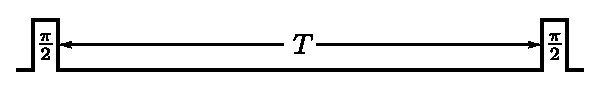
\includegraphics[width=1.95in]{figures_precreated/ramsey_sequence.eps}} & \imagetop{(a)} \\
	\imagetop{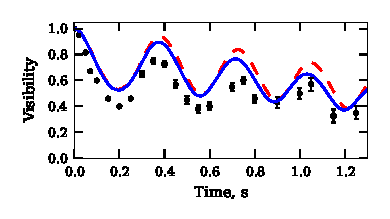
\includegraphics{figures_generated/ramsey_visibility.eps}} & \imagetop{(b)} \\
%	\vskip 0.2cm
	\imagetop{\hspace*{0.381in}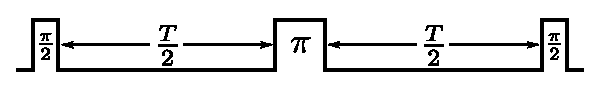
\includegraphics[width=1.95in]{figures_precreated/echo_sequence.eps}} & \imagetop{(c)} \\
	\imagetop{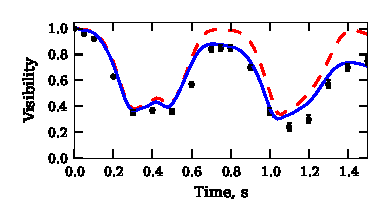
\includegraphics{figures_generated/echo_visibility.eps}} & \imagetop{(d)}
	\end{tabular}

	\caption{(color online).
	Timeline of the experiment for Ramsey (a) and Ramsey with symmetric spin-echo (c),
	(b) and (d) are the corresponding plots of interferometric visibility.
	Plots feature classical GPE calculations (red dashed lines),
	quantum noise simulations (solid blue lines) and
	experimental data (black circles).}

	\label{fig:visibility}
\end{figure}

The experiment consisted of preparation of stable BEC with state $\ket{1,+1}$ in a magnetic trap
and application of coupling electromagnetic pulses at certain times.
Two different schemes were used.
The first one was the simple Ramsey interferometry with $\pi/2$-pulse in the beginning,
evolution of resulting non-equilibrium superposition of states $\ket{1,+1}$ and $\ket{2,-1}$,
and the final $\pi/2$-pulse, which transformed the phase difference of the components
into the population difference (see~\figref{fig:visibility},~(a) for the timeline).
The second scheme had additional $\pi$-pulse (``spin-echo'') in the middle of the evolution,
which was supposed to partially restore interferometric contrast
(\figref{fig:visibility},~(c)).

\begin{figure}
	\begin{tabular}{l l}
	\imagetop{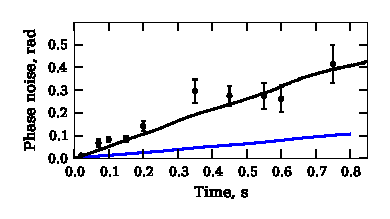
\includegraphics{figures_generated/ramsey_phnoise.eps}} & \imagetop{(a)} \\
	%	\vskip 0.2cm
	\imagetop{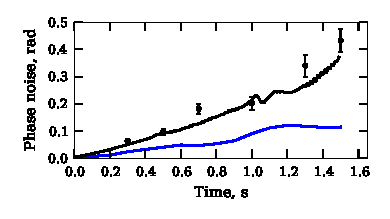
\includegraphics{figures_generated/echo_phnoise.eps}} & \imagetop{(b)}
	\end{tabular}

	\caption{(color online).
    Phase uncertainties for Ramsey (a) and spin echo (b) sequences.
    Contributions of local oscillator noise (dash-dotted lines),
	atom number uncertainty (dotted lines) and quantum noise (dashed lines)
	are shown along with their combined effect (solid lines).}

	\label{fig:phasenoise}
\end{figure}

	\bogdansremark{Should we note explicitly that Wigner method was used in Egorov et al. paper?}
	\petersremark{Yes, I think we should make a virtue of this, not hide it.
	As an example, of how to proceed, we can try to explore exactly
	how the spin-echo method improves the results.
	It is not exactly obvious how this works, and why it improves the results.
	A good numerical study may be able to shed light on this.}

We performed the calculations for these experiments using Wigner method and found that
it gives much better predictions than simulations with classical GPEs.
Wigner simulations have shown perfect results for spin-echo sequence (\figref{fig:visibility},~(d)),
although the fit for Ramsey sequence is not very accurate.
This can be explained, among other reasons, by the influence of classical noise,
which is eliminated in spin-echo sequence.
Comparison of experimentally measured phase noise and the noise given by simulations
(\figref{fig:phasenoise},~(a,~b)) confirms this;
the noise introduced by quantum effects is significantly smaller than the observed one.
Simulation results can be improved by the inclusion of ``classical'' noise sources,
such as frequency fluctuations of coupling pulses and uncertainty in the measured atom number
(their total effect is plotted as solid black lines on~\figref{fig:phasenoise}).

In conclusion, Wigner method of simulating BEC dynamics
is accurate enough for a range of interferometric experiments,
involving large numbers of atoms.
It is quite sensitive to the values of scattering lengths,
loss coefficients and some calculation parameters like the energy cutoff.
	\bogdansremark{Yes, downside was not the right word,
	but the sensitivity is something one should have in mind\---it is much more senitive to losses
	than GPEs are, and I bumped into this already.}

\bibliography{qsim}

\end{document}
